\chapter{LitQEval}\label{ch:ownApproach}
Despite ongoing research on automatic literature query generation and related evaluations with medical datasets, such as CLEF \autocite{kanoulas2017clef, kanoulas2018clef, kanoulas2019clef} and the Collection of Seeds \autocite{Wang_2022}, the insights gained from these evaluation metrics are not particularly compelling for our use case. This limitation arises from two main factors. 

First, the CLEF and Collection of Seeds datasets are exclusively focused on medical data. Although Badami's work \autocite{badami2023adaptive} offers a more diverse dataset, it lacks a suitable evaluation metric. Their evaluation primarily aims to maximize recall, with minimal consideration for precision, as literature search queries often yield far more results than necessary, making precision a less effective measure in this context. 

A second limitation arises when recall is prioritized exclusively. For example, if we aim to train a model to generate queries that maximize recall, there is no penalty for generating overly broad queries, such as those that exploit wildcards, which could lead to an excessive number of irrelevant results.

To address these issues, we introduce a dataset structured similarly to that of Badami \autocite{badami2023adaptive} but designed to be more comprehensive and covering a wider range of topics. Alongside this dataset, we propose new evaluation metrics that account for the inherently broad nature of literature search queries while penalizing excessively large queries. These metrics also emphasize the importance of accurately identifying core publications that are deemed highly relevant within the domain.


\section{Dataset}
The dataset we aim to create has three primary goals: First, it should encompass a wide range of randomly selected scientific research fields. Second, for each selected field, it should contain a set of highly relevant publications to serve as anchors for evaluating additional publications found in these areas. Lastly, the data should consider different research intents, meaning publication that is deemed relevant by a bibliometric analysis might not be relevant for a Systematic Literature Review (SLR) work.

Selecting new research topics is straightforward; however, to avoid bias from ongoing research interests, we used ChatGPT to generate a list of scientific fields that are recent and not overly broad. For instance, a topic like \textit{Artificial Intelligence} is vast, making it challenging to accurately and comprehensively identify core publications. Instead, we chose a more specific, problem-focused topics such as \textit{Drones in Agriculture}. To search for the corresponding bibliometric analysis we used the following query: \textit{<TERM>  ("Bibliometric" OR "Scientometric" OR "Systematic literature" OR "Most Influential" OR "Most Cited" OR "Scientific Landscape" OR "Literature Landscape" OR "Core Literature")} 


After identifying a sufficient number of diverse fields, 14 in our case, we sought to collect core publications for each field. Due to the difficulty of gathering core publications across a broad array of topics, we leveraged the bibliometrics community’s expertise. Specifically, we searched for bibliometric studies that identify the most relevant publications within each research area. For example, a bibliometric analysis of \textit{Drones in Agriculture} \autocite{Rejeb2022} lists the most cited publications from 1990 to 2021. In this case, 40 core publications were identified, which we manually located on Dimensions.ai and added to our dataset, omitting any publications not found in Dimensions.

This process was repeated across all selected research fields, resulting in a dataset comprising 14 topics, each containing 25–50 core publications, as shown in \autoref{fig:dataset-overview}. For the systematic literature review (SLR) data, we used previously collected data \autocite{badami2023adaptive} in the field of Software Engineering. Notably, the SLR data used here were replicated by executing the original query in Dimensions. However, only 7 out of the 10 original datasets were included, with SLR 2, 5, and 6 omitted due to extreme variations between the original datasets and the results retrieved from Dimensions. For instance, SLR 2 originally contained 8,911 candidate papers, but when executed in Dimensions, it yielded approximately 200,000. Overall, the dataset consists of 21 topics.


\begin{figure}
	\centering	
	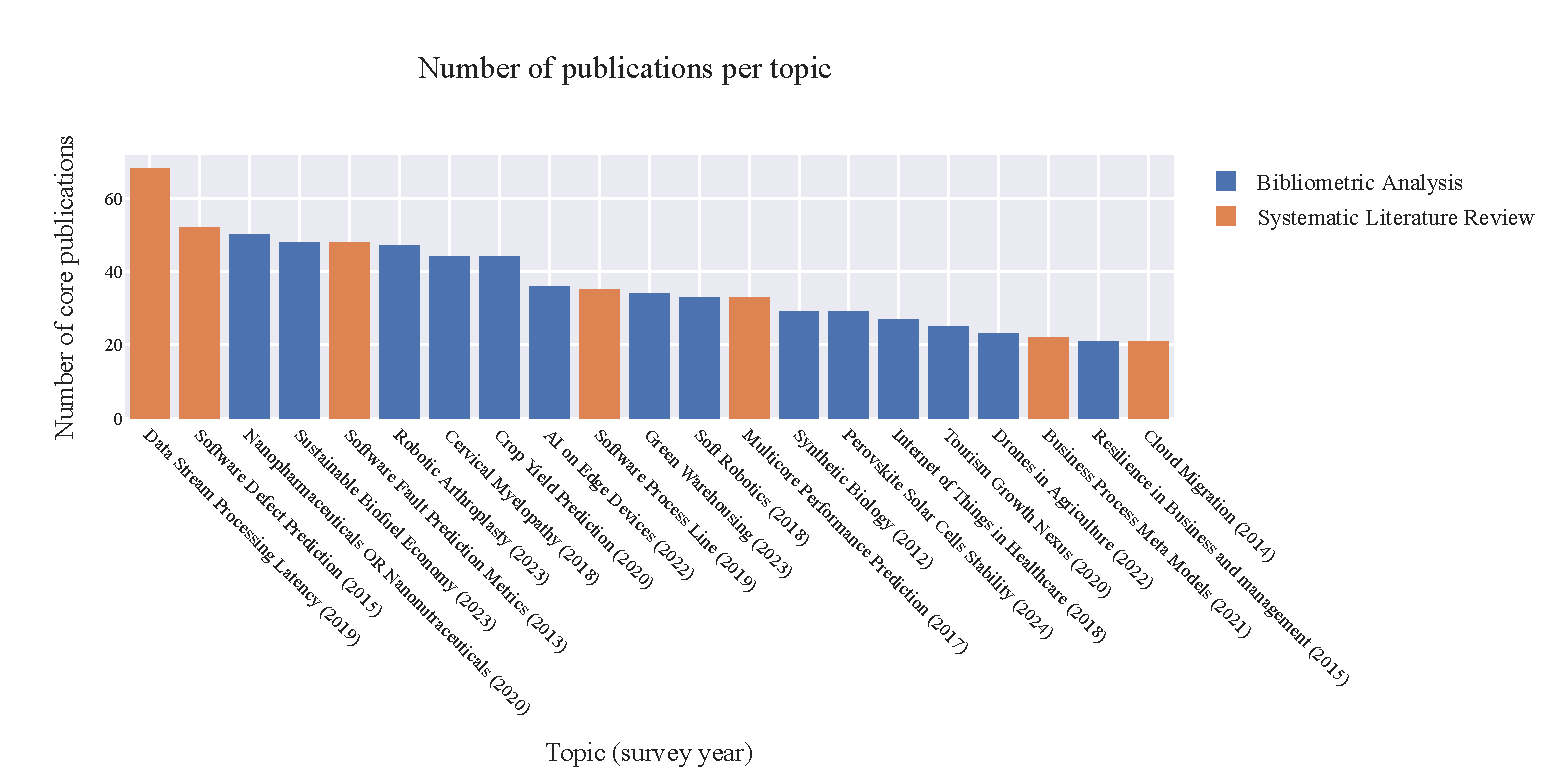
\includegraphics[scale=0.75]{pics/dataset-overview.pdf}
	\caption[Dataset overview of the research topics]{An overview of the dataset and the selected 21 research fields with respective core publications identified through bibliometric analyses or systematic literature review. The number in brackets following the field name on the x-axis represents the year of survey publication.}
	\label{fig:dataset-overview}
\end{figure}


\subsection{Dataset Analysis}

We recognize that potential biases may exist in our dataset due to its complete reliance on the bibliometric community for identifying core publications. This often implies that publications with higher citation counts are deemed more relevant. To assess this, we analyzed the citation distribution per topic, as provided by Dimensions, shown in \autoref{fig:dataset-citation}. Additionally, we examined the distribution of publication years per topic, illustrating the time span considered in the bibliometric analyses, as shown in \autoref{fig:dataset-years}.  If we compare the distribution of publication years for the medical research field \textit{Cervical Myelopathy} with that of \textit{IoT in Healthcare}, both of which were published in 2018, we can observe distinct differences in the year distributions of their core publications. These variations may be attributed to factors such as the recency of the field, changes in terminology over time, or the nature of the research area, where one field may prioritize more established works while the other focuses on recent advancements.


For the evaluation pipeline that we will introduce, the embeddings of the core documents are essential for effectively assessing the search query, as detailed in \autoref{sec:eval-metrics}. To validate this approach, we examine the clustered embeddings of the titles and abstracts for each core topic, as well as the bibliometric analyses in which these documents were initially referenced. This enables us to assess whether core publications within each field exhibit semantic similarity while also demonstrating some degree of dissimilarity from publications in other topics. The resulting clusters, shown in \autoref{fig:dataset-clustering}, were generated using k-means clustering, where $k$ is set to the number of topics. For this, we use OpenAI's small embeddings model alongside t-SNE\autocite{van2008visualizing} to reduce the dimensionality to 2D.

\begin{figure}
	\centering	
	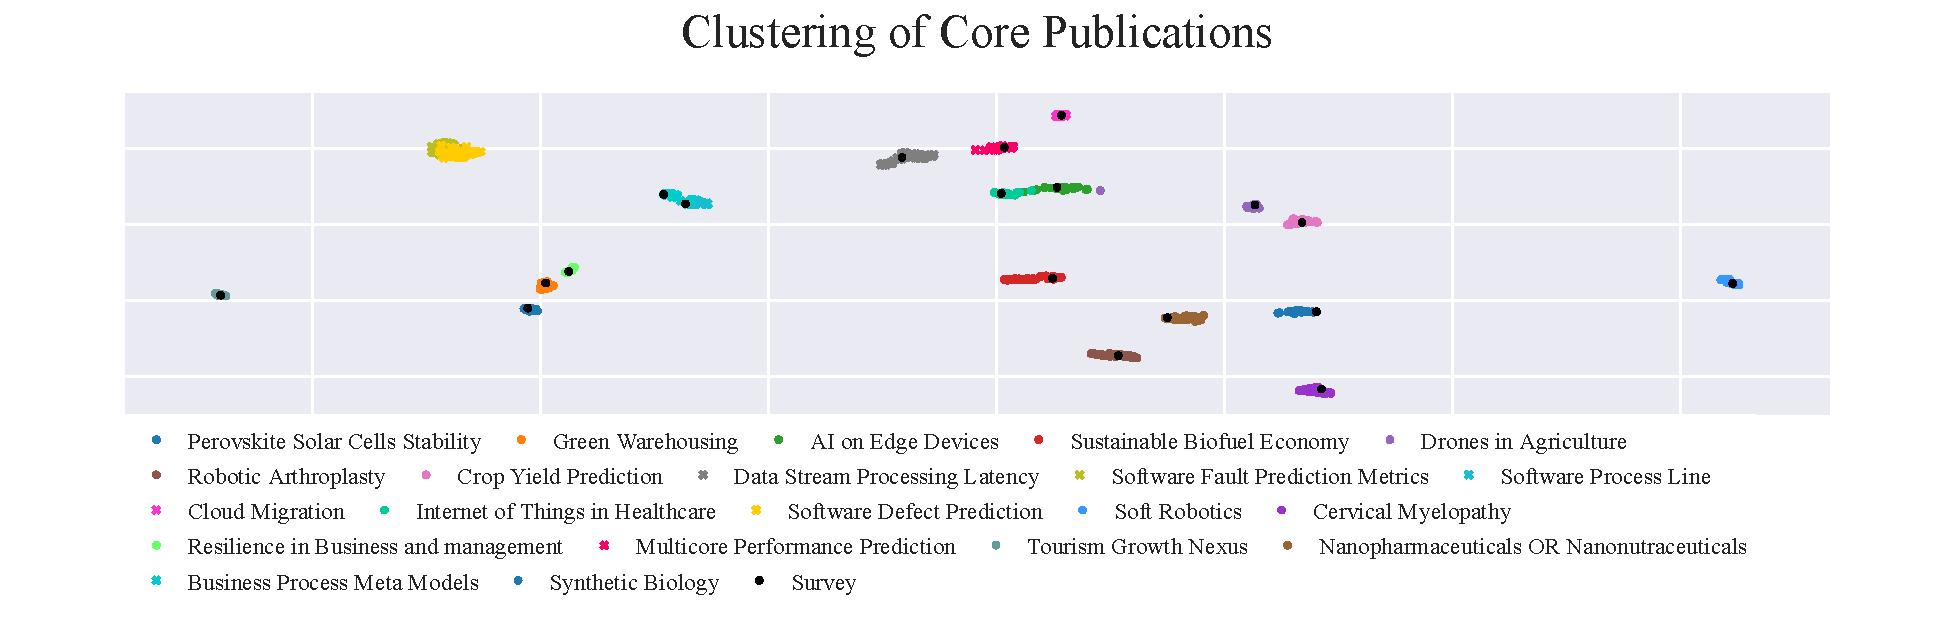
\includegraphics[scale=0.6]{pics/umap_clustering.pdf}
	\caption[Core Publications Clustering]{This figure shows clusters of publication embeddings based on titles and abstracts, the ones marked with o are from the BAs and X from SLRs . Embeddings were generated with OpenAI's small model and reduced in dimensionality with UMAP, then clustered using k-means with $k=21$ (indicating topic count). Clusters group core publications by semantic similarity, with overlaps in topics like \textit{IoT in Healthcare} and \textit{AI on Edge Devices}, as well as most of the SLR topic, due to the similarity in the research field.}
	\label{fig:dataset-clustering}
\end{figure}

\section{Evaluation metrics}\label{sec:eval-metrics}
The standard evaluation metrics for query evaluation are recall and precision. We argue that while recall is of high importance, particularly within the community, precision in this context becomes less feasible. Specifically, retrieving only the exact core publications via a search query would be impractical without explicitly using DOIs to target them directly, which renders this metric largely obsolete and likely to be consistently low. However, we still aim to account for the number of matched publications when executing a search query to prevent models from exploiting overly large queries. To address this, we introduce the concept of \textit{Semantic Precision}.

The idea behind Semantic Precision is to evaluate the relevance of retrieved publications in comparison to the core publication set. If the retrieved publications are sufficiently similar to those in the core set, they are deemed to hold some relevance rather than being entirely unrelated. To achieve this, we assume that the core publications, encompass sufficient semantic breadth to gauge the quality of literature relevant to a specific field. We calculate Semantic Precision in three ways.

\begin{figure}[]
	\centering	
	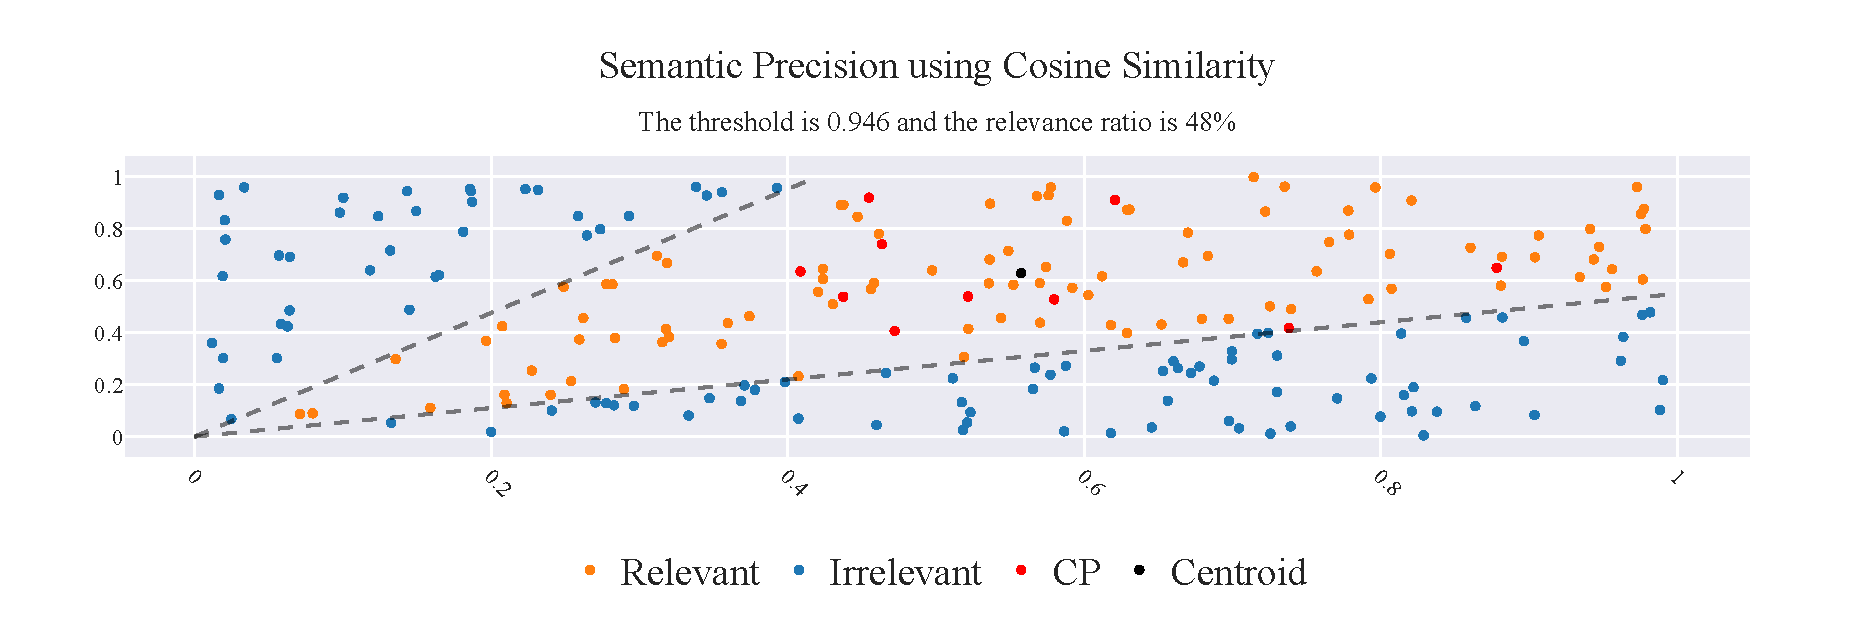
\includegraphics[scale=0.4]{pics/sp_cos.pdf}
	\caption[Semantic Precision using Cosine Similarity]{This illustration demonstrates the effect of cosine similarity on randomly generated data in a 2D space. The core publications (CP) are shown in red, positioned between 0.4 and 0.9 on both the x- and y-axes. When we set the threshold to 0.946, based on the cosine similarity of the least similar core publication from the centroid, many retrieved publications on the opposite side of the spectrum are still assigned as relevant. This effect occurs because cosine similarity considers only the angle between vectors, ignoring their magnitude. In this case, this results in 48\% of the retrieved publications being considered relevant.}

	\label{fig:sp-cos}
\end{figure}

\subsubsection{Semantic Cosine Precision}

The first approach involves averaging the embeddings of the core publications. We then set an acceptance threshold based on the cosine similarity to the least similar core publication, given by. This means that if the embedding of a retrieved publication is more similar to the center than the least similar core publication, we consider it a relevant publication, as shown in \autoref{fig:sp-cos}. We define:
\begin{itemize}
	\item $CPs$ as the set of core publications.
	\item $\vec{c_i}$ as the embedding vector of the $i$-th core publication.
	\item $\vec{p}$ as the embedding vector of a retrieved publication.
	\item $\cos(\vec{a}, \vec{b})$ as the cosine similarity between two vectors $\vec{a}$ and $\vec{b}$.
\end{itemize}

First, compute the centroid of the core publication embeddings:
\[
\vec{c}_{\text{centroid}} = \frac{1}{|CPs|} \sum_{\vec{c_i} \in CPs} \vec{c_i}
\]
Then, let the threshold similarity, $\theta$, be the cosine similarity of the least similar core publication to the centroid:
\[
\theta = \min_{\vec{c_i} \in CP} \cos(\vec{c}_{\text{centroid}}, \vec{c_i})
\]
Finally, Semantic Precision using cosine similarity ($SP_{cos}$) is defined as \autoref{eq:sp-cosine}, where $\mathbb{I}$ is an indicator function that equals 1 if the retrieved publication $\vec{r}$ meets the similarity criterion and 0 otherwise:
\begin{equation}\label{eq:sp-cosine}
	SP_{cos} = \frac{\sum_{\vec{p} \in \text{pubs}} \mathbb{I} \left( \cos(\vec{c}_{\text{centroid}}, \vec{p}) \geq \theta \right)}{|\text{retrieved}|}
\end{equation}

\begin{figure}[h!]
	\centering	
	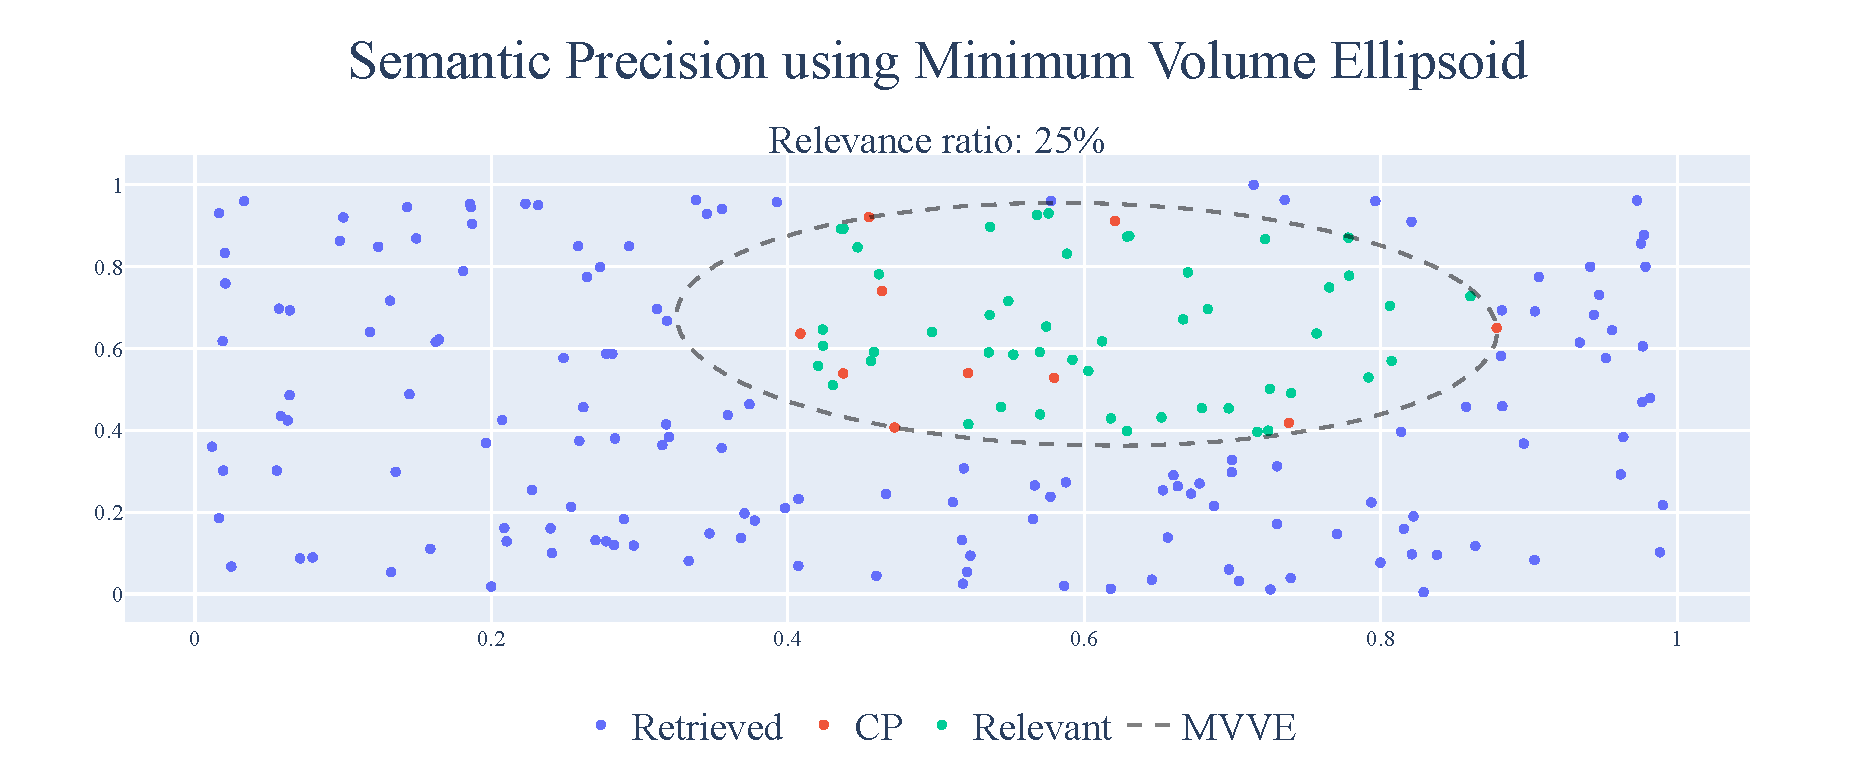
\includegraphics[scale=0.4]{pics/sp_mvee.pdf}
	\caption[Semantic Precision using MVEEE]{This illustration demonstrates the effect of using the Minimum Volume Enclosing Ellipsoid (MVEE) on randomly generated data in a 2D space. The core publications (CP) are shown in red, positioned between 0.4 and 0.9 on both the x- and y-axes. An ellipsoid is generated using MVEE to define the scope of relevant publications, ensuring that only those within the maximal angles and magnitudes of the core publications are considered relevant. In this case, this approach results in only 25\% of the retrieved publications being classified as relevant.}

	\label{fig:sp-mvee}
\end{figure}

\subsubsection{Semantic MVEE Precision}
For the second approach we omit the averaging of the embeddings and use Minimum Volume Enclosing Ellipsoid (MMVE), which creates the smallest ellipsoid that includes the our CP, which we then use to determine which of the retrieved publications are relevant by checking whether they are within MMVE or not, as illustrated in \autoref{fig:sp-mvee}. This approach allows us to take into account all the dimensions by not only considering the angle but also the magnitude

The Minimum Volume Enclosing Ellipsoid (MVEE) for the core publication set $CP$ is centered at $\delta$ with shape matrix $A$. To determine whether a retrieved publication $\vec{r}$ is relevant, we check if it lies within the ellipsoid by testing the following condition:
\[
(\vec{p} - \delta)^T A (\vec{p} - \delta) \leq 1
\]
Semantic Precision (SP) for this approach is then:

\begin{equation}\label{eq:sp-mvee}
	\text{SP}_{\text{MVEE}} = \frac{\sum_{\vec{p} \in \text{pubs}} \mathbb{I} \left( (\vec{p} - \delta)^T A (\vec{p} - \delta) \leq 1 \right)}{|\text{pubs}|}
\end{equation}

Additionally, it is also possible to use a convex hull, which is the smallest convex set that encloses all the points by forming a polygon. A potential advantage of this approach is that it is more robust to outliers compared to the Minimum Volume Enclosing Ellipsoid (MVEE).

\subsubsection{Semantic Clustering Precision}

For the final semantic precision approach, we apply a simple clustering algorithm, such as k-means, on the document embeddings. The process iteratively adjusts the number of clusters \( K \), starting with \( K=2 \), and increases \( K \) until a specific condition is met. We define a threshold \( \theta \) that determines the stopping criterion based on the number of core publications in the smallest cluster. Specifically, we stop when the number of core publications (\( CPs \)) in the smallest cluster satisfies the condition:
\begin{equation}
CPs \text{ in cluster smallest cluster} \leq \theta \cdot \text{Maximum possible } CPs
 \end{equation}\label{eq:sp-clustering}
This ensures that the smallest cluster contains at least \( \theta \) of the core publications.
All the above semantic precision metrics aim to identify potential true positives that were initially not considered as \( CPs \). However, a key issue arises when the number of semantically relevant publications is large due to the broad scope of the initial query. 

For instance, if a query retrieves 50,000 publications, with 30,000 deemed relevant, this still poses a challenge. Screening such a large volume of documents is infeasible, making the results problematic. To address this, we introduce a decay factor to the semantic precision, defined as follows:

\begin{itemize}
	\item \( p \): Controls the initial slowness of the decay.
	\item \( q \): Controls the acceleration of the decay near the end.
	\item $\alpha$: The maximum threshold for the decay, representing the point at which the decay becomes negligible.
\end{itemize}

The decay function is expressed as:

\[
\lambda = \left(1 - \left(\frac{n_{\text{pubs}}}{\alpha}\right)^p\right)^q
\]


\begin{figure}[h!]
	\centering	
	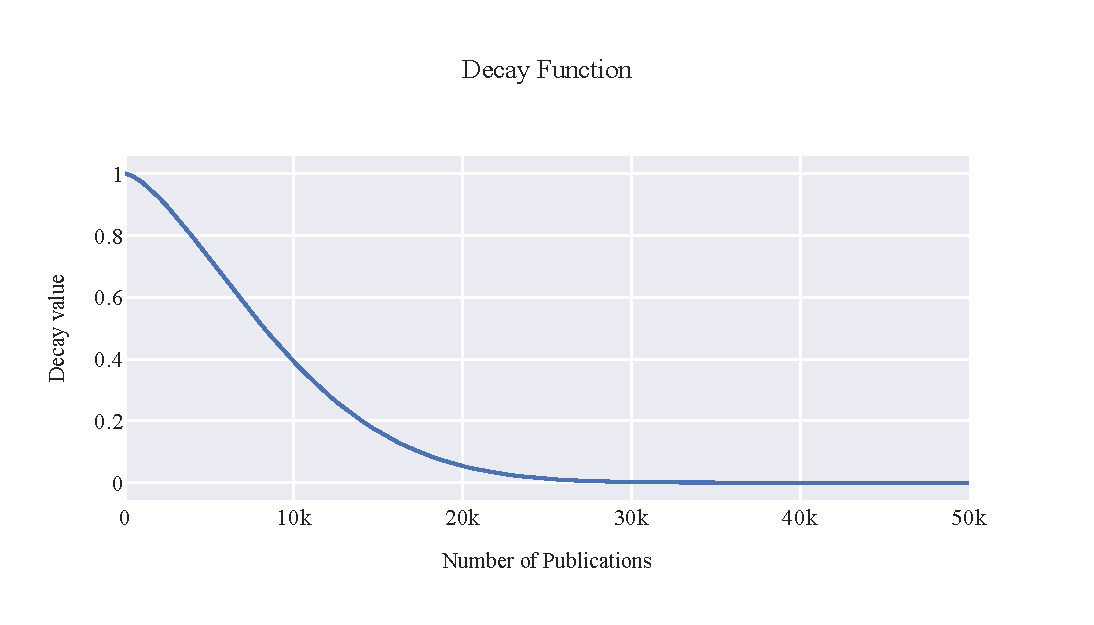
\includegraphics[scale=0.7]{pics/decay_function.pdf}
	\caption[Decay function for semantic precision]{This illustration demonstrates the effect of the decay factor, which ensures that the contribution of a large number of publications diminishes as the total count approaches the threshold. This prevents an overwhelming volume from biasing the semantic precision. For this example, we set the threshold (\( \alpha \)) to 50k, \( p=1.5 \), and \( q=10 \).}	
	\label{fig:decay-function}
\end{figure}


Now that we have metrics that can be used penalizes the model in case of generating a too broad of a query, we use can use it as a factor to calculate the F-Score, the goal of the standard F-score is to balance out between the recall and precision, but in our case we use $F-\beta$ instead, whereby the $\beta$ is the weighting factor of the recall, meaning the higher it is the more important the recall will be, in our case we set it to be 2, meaning that the recall is twice as important as the precision.
\begin{equation}\label{eq:f-beta}
F_\beta = (1 + \beta^2) \cdot \frac{\text{Precision} \cdot \text{Recall}}{(\beta^2 \cdot \text{Precision}) + \text{Recall}}
\end{equation}
For our specific case where $\beta = 2$, emphasizing the importance of recall, it is:
\[
	F_2 = 5 \cdot \frac{(\text{Precision} \cdot \lambda) \cdot \text{Recall}}{(4 \cdot \text{Precision}\cdot \lambda) + \text{Recall}}
\]

\subsection{Comparative Analysis}

To further understand the metrics and their impact on evaluating the dataset, we conduct an in-depth analysis using a randomly selected topic, \textit{Soft Robotics} and used its baseline query as a case study. First, we visualize the embeddings of the baseline and predicted queries \autoref{fig:sr-landscape}. The baseline query is the exact topic name, \textit{Soft Robotics}, while the predicted query is generated by the SQW. The embeddings are derived from the title and abstract of the retrieved publications and subsequently reduced to a 2D UMAP \autocite{mcinnes2020umap} space. It is important to note that a significant amount of information is likely lost due to the extreme dimensionality reduction from 1536 dimensions to 2.


\begin{figure}[!ht]
	\centering	
	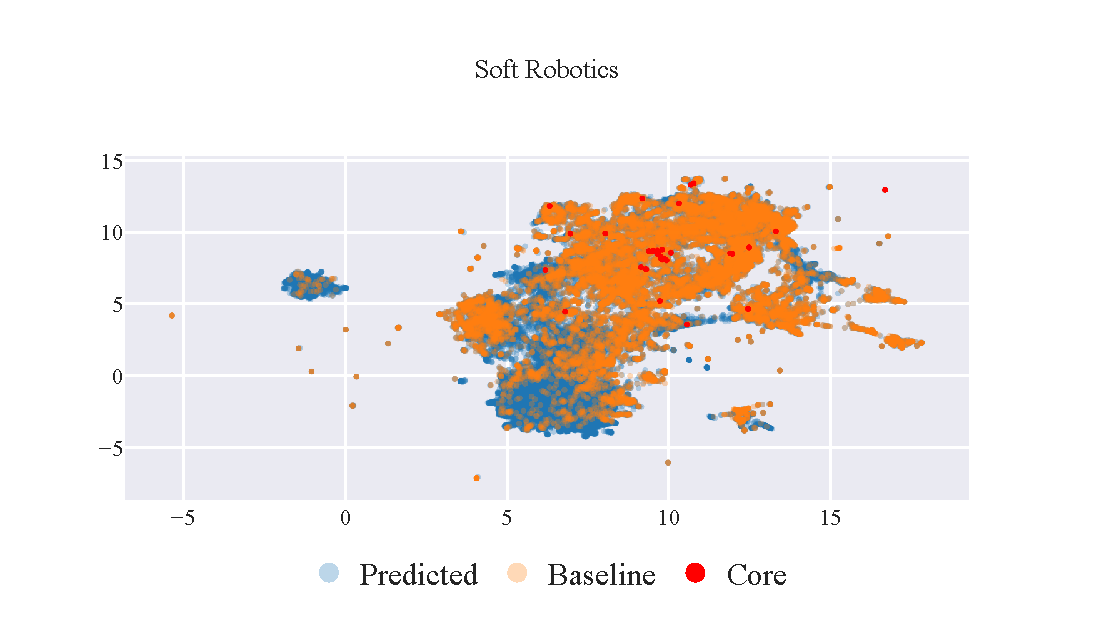
\includegraphics[scale=0.7]{pics/sr-landscape.pdf}
	\caption[Embedding of Soft Robotics]{This figure visualizes the distribution of publications retrieved by both the baseline and predicted queries in a 2D space. The baseline query retrieved 20 core publications, whereas the predicted query retrieved 26 core publications out of a total of 36.}\label{fig:sr-landscape}
\end{figure}

\subsubsection{Semantic Cosine Precision}
At first, we test the Semantic Cosine Precision using the high-dimensional original embedding $E_o$, which was done as described in \autoref{eq:sp-cosine}. This resulted in 13,265 out of 17,573 publications being classified as relevant \autoref{fig:sr-cosine-baseline}. However, this high proportion of relevant publications appeared excessive, prompting further investigation into the threshold's effect on the number of semantically relevant documents.

Since we aim to use the $F_2$ score as our primary evaluation metric, we also employed it as a cost function to maximize. The goal was to identify the optimal empirical threshold that balances the retrieval of core publications with the number of relevant publications. To achieve this, we used the inverse precision, defined as $\frac{\text{Total Retrieved Publications}}{\text{Number of Relevant Publications}}$, instead of standard precision. The results \autoref{fig:threshold-analysis} reveal that a threshold maximizing the number of retrieved core publications while minimizing false positives is approximately 0.69. This suggests that sometimes sacrificing a couple of core publications is rewarding because it allows us to reduce the total number of semantically relevant publications.

\begin{figure}
	\centering	
	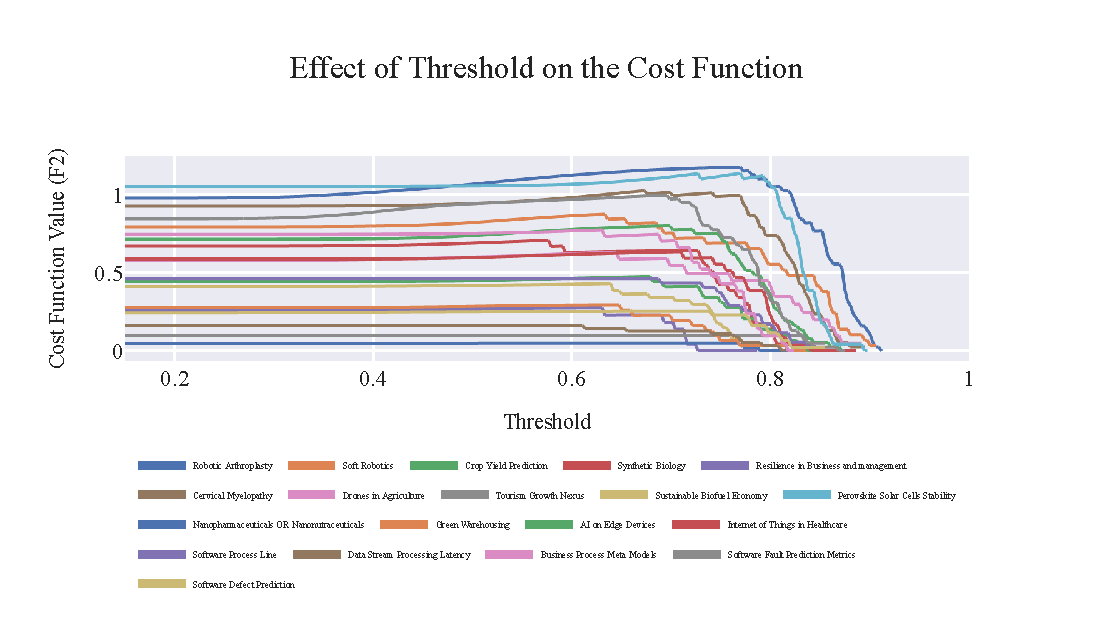
\includegraphics[scale=0.7]{pics/threshold-analysis.pdf}
	\caption[Semantic Cosine Threshold: Empirical Analysis]{This figure illustrates the effect of the threshold on the $F_2$ score. As the threshold increases, the number of semantically relevant publications and core publications identified decreases. However, in some cases, such as \textit{Perovskite Solar Cells Stability}, the $F_2$ score continues to improve despite the loss of a core publication. This outcome is due to the $F_2$ score weighting recall twice as much as precision, allowing for stricter relevance criteria while sacrificing a single core publication.}\label{fig:threshold-analysis}
\end{figure}

After setting the threshold to the optimal empirical value, the Semantic Cosine Precision retrieves 19 out of the initially found 20 core publications while significantly reducing the number of semantically relevant publications by a factor of 4. This adjustment results in only 3,424 publications being identified as relevant, compared to the initial 13,265. However, this refinement comes at the cost of missing one core publication.

\subsubsection{Semantic MVEE Precision}

In contrast to Semantic Cosine Precision, we opt to use the 2D embeddings generated by UMAP $E_{umap}$, rather than the original high-dimensional embeddings, $E_o$. This decision was made because earlier evaluations of the dataset showed that the MVEE consistently classified at least 50\% of the total retrieved documents as relevant, which we believe is related to the high-dimensional nature of the embedding vectors.

We experiment with two enclosing shapes: the MVEE and a Convex Hull. The primary difference is that the MVEE tends to be larger due to its ellipsoidal shape, whereas the convex hull strictly bounds the points. Using the MVEE approach, 9,595 publications were identified as relevant out of the total 17,573 publications, as shown in \autoref{fig:sr-mvee-baseline}. In contrast, the convex hull, being smaller as expected, identified 7,609 publications as relevant, as illustrated in \autoref{fig:sr-hull-baseline}.

\begin{figure}
	\centering	
	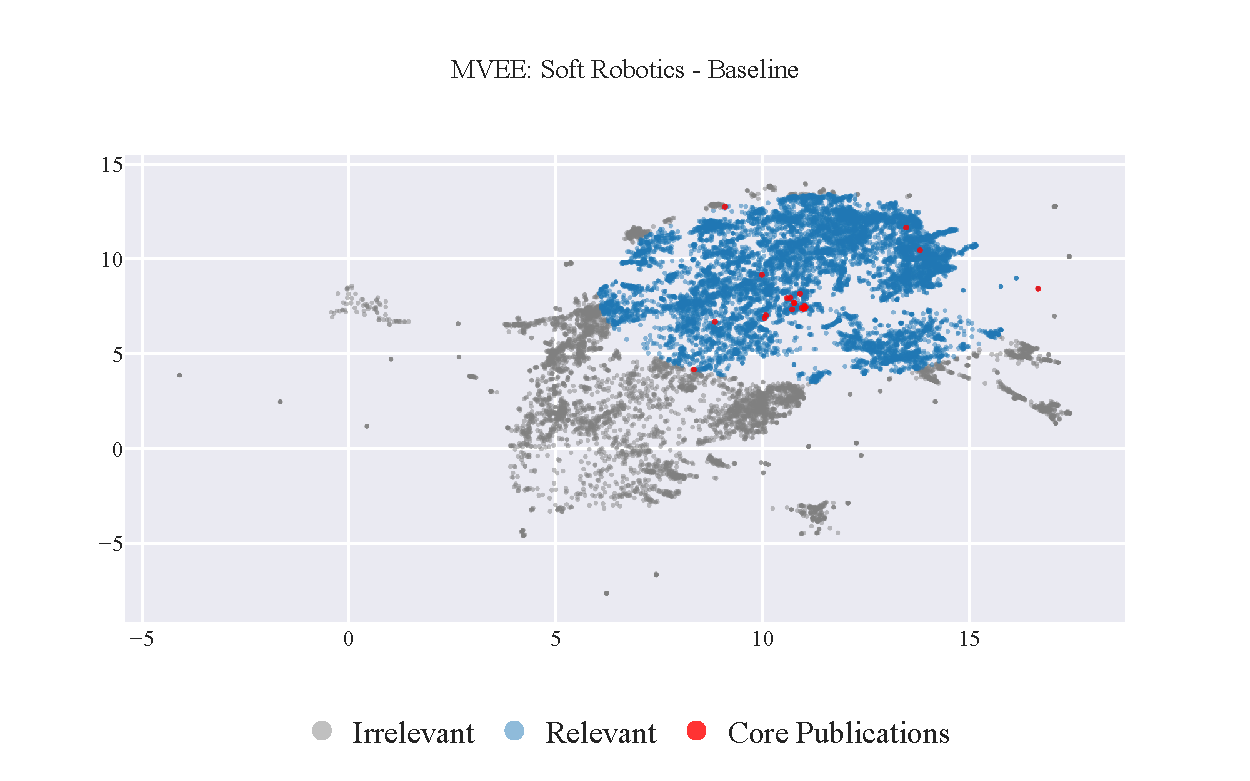
\includegraphics[scale=0.6]{pics/sr-mvee-baseline.pdf}
	\caption[Semantic MVEE: Soft Robotics]{This figure shows the relevant publications identified by the Minimum Volume Enclosing Ellipsoid (MVEE). An advantage of this approach is that we always expect that all teh core publications to be included in the identified publications.}\label{fig:sr-mvee-baseline}
\end{figure}

For further evaluation, understanding the quality of the UMAP embeddings ($E_{UMAP}$) is crucial, as they do not retain the same level of semantic meaning as the original higher-dimensional embeddings ($E_o$). Unlike PCA, which is a linear transformation, calculating the exact semantic loss for UMAP embeddings is challenging due to its nonlinear nature. To approximate this loss, we utilized a Partial Least Squares Regression approach as outlined by Oskolkov\footnote{\url{https://towardsdatascience.com/umap-variance-explained-b0eacb5b0801}}. Based on this method, we estimated that the explained variance of the two-dimensional UMAP embeddings is only 7.15\%. This low explained variance underscores the significant reduction in information captured when transitioning from high-dimensional to two-dimensional space.


\subsubsection{Semantic Clustering Precision}

To cluster the embeddings, we use K-means for $2 \leq K \leq 100$, iteratively determining the smallest possible cluster containing at least 70\% of the core publications which is the threshold $\theta$ described in \autoref{eq:sp-clustering}. For this process, we use the high-dimensional embeddings, $E_o$, as input. Cosine similarity is used as the distance measure between points which requires input normalization, which is already facilitated by the output of OpenAI's text-embedding-3-small model.

\begin{figure}[!hb]
	\centering	
	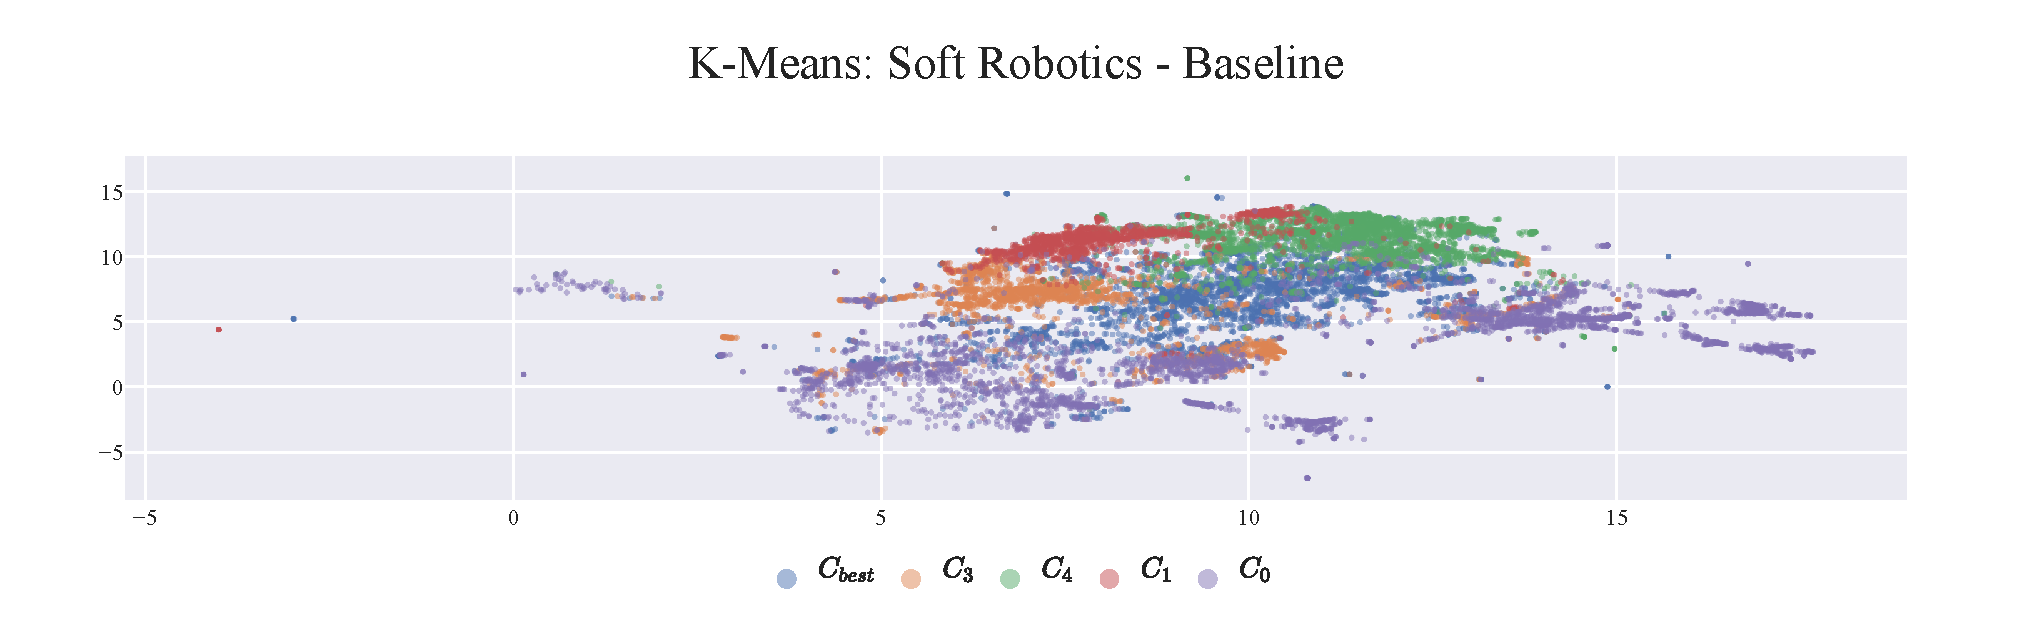
\includegraphics[scale=0.6]{pics/sr-clustering-baseline.pdf}
	\caption[Semantic Clustering: Soft Robotics]{This illustration shows the grouping of the embeddings $E_o$ in higher-dimensional space using K-means with $K = 0, 1, 2, 3, 4,$ and $5$, where $K=5$ is identified as the optimal solution. The spread-out nature of the clusters is uncommon in K-means but occurs here because clustering is performed in the higher-dimensional space before reducing the data to 2D using UMAP for visualization.}\label{fig:sr-clustering-baseline}
\end{figure}

The clustering results \autoref{fig:sr-clustering-baseline} indicate that the space can be divided into 5 groups. The best group has a size of 4,954 out of 17,573 publications and contains 15 out of the 20 core publications. We experimented with adjusting the threshold to match the quality of cosine similarity by increasing it to the next best solutions. At a threshold of approximately 0.75, the results included 6,861 publications with 17 core publications. At a threshold of approximately 0.85, all 17,573 publications were clustered together.

Additionally, we clustered the UMAP embeddings, $E_{UMAP}$, using the same thresholds (0.7, 0.75, and 0.85). These thresholds consistently yielded similar results, with 11,644 out of 17,573 publications identified as relevant and 19 out of the 20 core publications included. This consistency can serve as an indicator of the information loss incurred when using UMAP.

As mentioned in \autoref{sec:eval-metrics}, the $F_{\beta}$ score is the metric we will use for evaluation, with $\beta=2$, emphasizing recall by making it twice as important as precision. However, we extend the traditional $F_{\beta}$ score by incorporating components such as semantic precision in place of typical precision and introducing a decay factor to account for the number of semantically relevant retrieved publications. To better understand the influence of each component, we visualize their effects in \autoref{fig:f-score}.

\begin{figure}[!hb]
	\centering	
	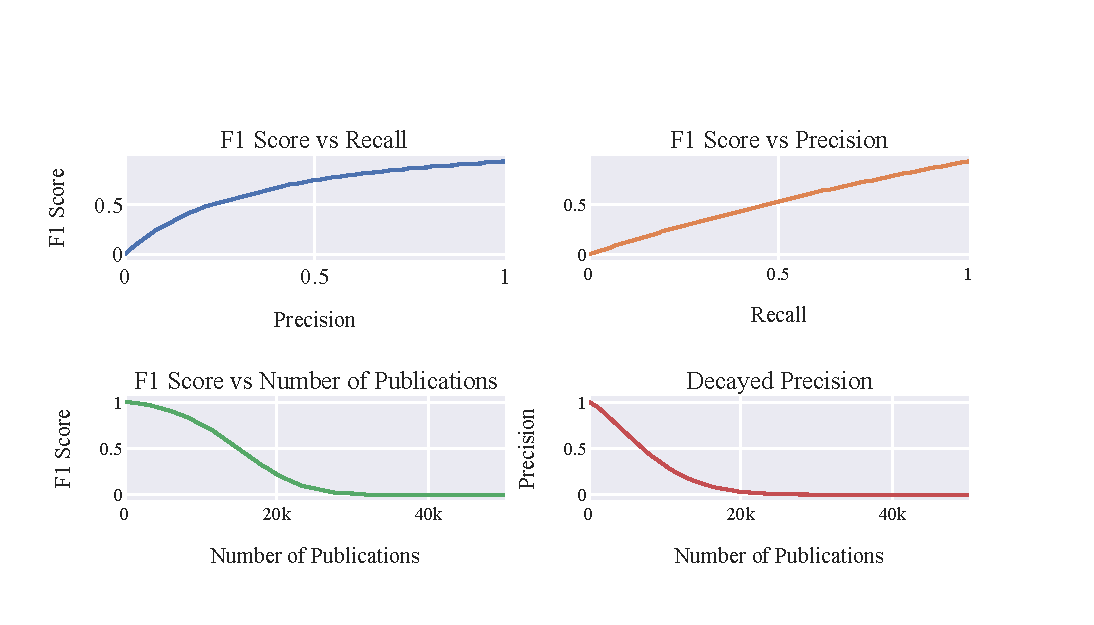
\includegraphics[scale=0.7]{pics/f_score.pdf}
	\caption[$F_{\beta}$ components analysis]{This illustration demonstrates the effect of each component in the $F_{\beta}$ score evaluation metric, where $\beta=2$ and the decay hyperparameters are set to $p=1.5$, $q=10$, and $\alpha=50000$. In the top left, we observe the impact of $\beta=2$, which ensures better scaling even with lower precision if the recall is 1. The top right plot shows how the score scales almost linearly with the precision. The bottom left and right plots depict the dampening effect on the $F_{\beta}$ score as the number of relevant publications increases, emphasizing the importance of controlling the decay to prevent inflated scores from overly large results.}\label{fig:f-score}
\end{figure}

